%&pdflatex
\documentclass[smallextended, referee]{svjour3} % svjour3: smallextended, referee
\usepackage[english]{babel}
\usepackage[T1]{fontenc}
\usepackage{graphicx}
\usepackage{amssymb, amsmath}
\usepackage{endfloat}
\usepackage{cite}
\usepackage{fixltx2e}
\usepackage{fullpage}

\newcommand{\Kn}{\mathrm{Kn}}
\newcommand{\dd}{\:\mathrm{d}}
\newcommand{\pder}[2][]{\frac{\partial#1}{\partial#2}}
\newcommand{\pderder}[2][]{\frac{\partial^2 #1}{\partial #2^2}}

\journalname{Theoretical and Computational Fluid Dynamics}

\begin{document}

\title{
	Computer simulation of a stationary gas in the continuum limit with considerable temperature gradients
}

\author{O.A.~Rogozin}
\institute{O.A.~Rogozin \at
	Moscow Institute of Physics and Technology,
	9 Institutskiy pereulok, g. Dolgoprudny,
	Moskovskaya obl., Russian Federation\\
	\email{o.a.rogozin@gmail.com}  
}

\maketitle

\begin{abstract}
	Classical fluid dynamics describes a behavior of gas in terms of the compressible Navier--Stokes
	set of equations. However, a rigorous asymptotic analysis of the Boltzmann equation confines
	the scope of its application and leads to a more complicated set of differential equations,
	for example, when large temperature gradients are present. Based on the CFD platform
	OpenFOAM\textregistered{} a special parallel solver is designed for numerical simulation of a slightly rarefied gas
	in an arbitrary geometry with a finite Reynolds number. Considered two-dimensional problems
	clearly illustrate significant flows eluding from the solution of the conventional equations.
	\keywords{
		numerical simulation \and Boltzmann equation \and Navier--Stokes equations \and thermal creep flow \and
		nonlinear thermal-stress flow \and ghost effect
	}
	\PACS{47.45.-n,47.11.Df}
\end{abstract}

\section{Introduction}

Let us consider a gas with a small mean free path in a closed vessel in the absence of gravity.
For gas in the equilibrium state at rest, temperature field is governed by the heat-conduction equation.
However, using the no slip boundary condition for the compressible Navier--Stokes set of equations
is not valid if the vessel walls have a large temperature variation~\cite{Kogan1976, GhostEffect}.
The correct equations on the macroscopic variables can be obtained from the asymptotic theory of
the Boltzmann equation~\cite{Sone2002, Sone2007}.

This new set of equations has the similar structure to the Navier--Stokes one,
so appropriate numerical methods are formulated on the same principles that accepted in CFD.
The first solutions presented in literature are based on the finite difference methods~\cite{GhostEffect, SoneCoaxial}.
Following works treat with the finite volume methods~\cite{Laneryd2006, Laneryd2007}.
The next stage is a parallel implementation of these numerical methods that allows
to solve complex engineering problems.

One of the modern CFD platforms, OpenFOAM\textregistered{}~\cite{OpenFOAM1998, OpenFOAM2010} has
already an active endeavor to widen its scope to rarefied gas dynamics~\cite{Pantazis2012}.
In the present work a parallel solver was developed within this open-source platform.
The program code validation was carried out by means of some benchmark simulations,
presented as illustrations in this paper.

First, we outline the basic equations and the key points of the asymptotic theory,
used in the implementation of the program solver.
Then we present the results of numerical simulation for some specific problems
and compare the obtained temperature fields to the classical solution
of the heat-conduction equation.

\section{The basic equations}

Liquids and gases are described by the conservation laws of mass, momentum and energy:
\begin{gather}
	\pder[\rho]{t} + \pder{x_i}(\rho v_i) = 0, \label{eq:mass}\\
	\pder{t}(\rho v_i) + \pder{x_j}(\rho v_i v_j + p_{ij}) = \rho F_i, \label{eq:momentum}\\
	\pder{t}\left[\rho\left(e+\frac{v_i^2}2\right)\right] +
		\pder{x_j}\left[\rho v_j\left(e+\frac{v_i^2}2\right)+v_i p_{ij}+q_j\right] = \rho v_j F_j. \label{eq:energy}
\end{gather}
Macroscopic variables have the following notation: the density \(\rho\), the flow velocity \(v_i\), the stress tensor \(p_{ij}\),
the specific internal energy \(e\), and the heat-flow vector \(q_i\). Finally, \(F_i\) denotes the external force.
For an ideal monatomic gas, the internal energy \(e\) depends only on the temperature \(T\):
\[ e = \frac32RT, \]
where \(R = k_B / m\) is the specific gas constant. The pressure is taken from the equation of state:
\[ p = \rho RT. \]

The conservation equations are closed to the Navier--Stokes set by means of the Newton and Fourier laws
for the stress tensor \(p_{ij}\) and the heat-flow vector \(q_i\), respectively:
\begin{gather}
	p_{ij} = p\delta_{ij} - \mu\left(\pder[v_i]{x_j}+\pder[v_j]{x_i}-\frac23\pder[v_k]{x_k}\delta_{ij}\right) -
		\mu_B\pder[v_k]{x_k}\delta_{ij}, \label{eq:stress_tensor}\\
	q_i = -\lambda\pder[T]{x_i}. \label{eq:heat_flow}
\end{gather}
Transport coefficients are given above:
the viscosity \(\mu\), the second viscosity \(\mu_B\), and the thermal conductivity \(\lambda\).

A Knudsen number \(\Kn\) is determined by the ratio of the mean free path
\begin{equation}\label{eq:ell}
	\ell = \frac{m}{\sqrt2\pi d_m^2 \rho}.
\end{equation}
to the characteristic dimension of the problem \(L\):
\begin{equation}\label{eq:Knudsen}
	\Kn = \frac{\ell}L.
\end{equation}
It is convenient to deal with a modified Knudsen number:
\begin{equation}
	k = \frac{\sqrt\pi}2\Kn.
\end{equation}
For a hard-sphere gas, the radius of the intermolecular force influence \(d_m\)
coincides with the diameter of a molecule.

Further variables are assumed dimensionless with corresponding reference units:
the length \(L\), the pressure \(p^{(0)}\), the temperature \(T^{(0)}\),
the velocity \((2RT^{(0)})^{1/2}\) and the heat-flow vector \(p^{(0)}(2RT^{(0)})^{1/2}\).

The viscosity \(\mu\) and the thermal conductivity \(\lambda\) of an ideal gas
are proportional to the mean free path \(\ell\), and thus to the Knudsen number:
\begin{equation}
	\mu = O(k), \quad \lambda = O(k).
\end{equation}
For \(k\to0\) we obtain the Euler set of equations:
\begin{equation}
	p_{ij} = p\delta_{ij}, \quad q_i = 0.
\end{equation}

However, the Euler set failed to determine the temperature field.
Classical heat-conduction equation is derived from~\eqref{eq:energy} and~\eqref{eq:heat_flow}
in the absence of gas motion \(v_i = 0\):
\begin{equation}\label{eq:heat_equation}
	\pder{x_i}\left(\sqrt{T}\pder[T]{x_i}\right) = 0.
\end{equation}
It takes into account that the thermal conductivity of an ideal gas is proportional to \(\sqrt{T}\).

For small \(k\) weak convective flow \(v = O(k)\) appears in the Navier--Stokes set of equations.
It compensates a thermal conductivity term in~\eqref{eq:energy}.
Despite its disappearance for \(k\to0\), it has a finite influence on the temperature field.
This finite effect produced by an infinitesimal quantity is called \textit{ghost effect}~\cite{Sone2002}.
It can be described only within the kinetic theory framework treating the asymptotic behavior of
the Boltzmann equation for small Knudsen numbers.

\section{The asymptotic analysis of the Boltzmann equation}
A detailed mathematical derivation of the following results can be found in~\cite{Sone2002, Sone2007}.

The analysis presented below is based on the conventional Hilbert expansion~\cite{Hilbert1912}
of the distribution function \(f\) and the macroscopic variables \(h\):
\[ f = f_0 + f_1k + f_2k^2 + \cdots, \]
\[ h = h_0 + h_1k + h_2k^2 + \cdots \]
with the additional condition
\begin{equation}\label{eq:Mach_constraint}
	\int\xi_if\dd\xi = O(k),
\end{equation}
meaning that the Mach number is of the same order as the Knudsen number.

The outcome embodies the following set of equations for stationary variables \(T_0\), \(u_{i1} = p_0v_{i1}\), \(p_2\):
\begin{align}
	\pder{x_i}\left(\frac{u_{i1}}{T_0}\right) &= 0, \label{eq:asymptotic1} \\
	\pder{x_j}\left(\frac{u_{i1}u_{j1}}{T_0}\right)
		&-\frac{\gamma_1}2\pder{x_j}\left[\sqrt{T_0}\left(
			\pder[u_{i1}]{x_j}+\pder[u_{j1}]{x_i}-\frac23\pder[u_{k1}]{x_k}\delta_{ij}\right
		)\right] \notag\\
		&- \frac{\gamma_7}{T_0}\pder[T_0]{x_i}\pder[T_0]{x_j}\left(\frac{u_{j1}}{\gamma_2\sqrt{T_0}} - \frac{1}4\pder[T_0]{x_j}\right) \notag\\
		&= -\frac1{2p_0}\pder[p_2^\dag]{x_i}, \label{eq:asymptotic2} \\
	\pder[u_{i1}]{x_i} &= \frac{\gamma_2}2\pder{x_i}\left(\sqrt{T_0}\pder[T_0]{x_i}\right). \label{eq:asymptotic3}
\end{align}
Pressures \(p_0\) and \(p_1\) are constant,
\[ 
	p_2^\dag = p_2 + 
		\frac{2\gamma_3}{3p_0}\pder{x_k}\left(T_0\pder[T_0]{x_k}\right) -
		\frac{\gamma_7}{6p_0}\left(\pder[T_0]{x_k}\right)^2,
\]
The set of equations \eqref{eq:asymptotic1}--\eqref{eq:asymptotic3} has a fluid-dynamic nature
and is comparable to the Navier--Stokes equations for a compressible gas (\(\rho_0 = p_0/T_0\)).
The formal difference consists in the additional thermal stress terms.
Moreover, \(p_2^\dag\) is not included in the equation of state, therefore is determined up to a constant.
Term \(\partial{p_2 ^ \dag} / \partial{x_i}\) participates in the system as the pressure
in the Navier--Stokes set for incompressible gas.
This fact determines the corresponding numerical methods for solving the above system.

For a hard-sphere gas, dimensionless transfer coefficients are equal
\begin{alignat*}{2}
	\gamma_1 &= 1.270042427, &\quad \gamma_2 &= 1.922284066, \\
	\gamma_3 &= 1.947906335, &\quad \gamma_7 &= 1.758705.
\end{alignat*}

The first two ones correspond to the viscosity and the thermal conductivity:
\[ \mu = \frac{\sqrt\pi}2\gamma_1, \quad \lambda = \frac{5\sqrt\pi}2\gamma_2. \]

The fluid-dynamic boundary conditions based on the diffuse-reflection boundary conditions
for Boltzmann equation look as follows:
\begin{gather}
	T_0 = T_w, \label{eq:bound:T} \\
	\left\{
	\begin{aligned}
		& \frac{(u_{j1}-u_{wj1})}{\sqrt{T_w}}(\delta_{ij}-n_in_j) = 
			-K_1\pder[T_w]{x_j}(\delta_{ij}-n_in_j), \\
		& u_{j1}n_j = 0.
	\end{aligned}
	\right. \label{eq:bound:v}
\end{gather}
Here \(n_i\) is the normal to the surface, \(u_{wj1}\), \(T_w\) are the velocity and the temperature of the boundary.
\(K_1\) is the dimensionless coefficient for the thermal creep. For a hard-sphere gas
\[ K_1 = -0.6463. \]

In the general case, the solution of the boundary-value problem cannot be expressed only
with the fluid-dynamic-type solution due to the sharp variation in the distribution function
near the boundary.
It is therefore necessary to introduce the so-called Knudsen-layer correction:
\begin{equation}
	f = f_{FD} + f_K.
\end{equation}
The fluid-dynamic part \(f_{FD}\) is the solution presented above,
and \(f_K\) decays exponentially with the distance to the boundary \(\eta\):
\begin{equation}
	f_K = O\left(e^{-\eta}\right), \quad \eta = \frac{x_in_i}k.
\end{equation}

Due to the infinitesimal Mach number (\ref{eq:Mach_constraint}) \(f_K\) is expanded
in a power series of \(k\), starting from the first order:
\[ f_K = f_{K1} k + f_{K2} k ^ 2 + \cdots \]
The Knudsen layer introduces a correction to \(u_{i1}\) for a hard-sphere gas:
\begin{equation}
	\left\{
	\begin{aligned}
		& \frac{u_{jK1}}{\sqrt{T_w}}(\delta_{ij}-n_in_j) = 
			-\frac12\pder[T_w]{x_j} Y_1\left(\frac\eta{T_w}\right) (\delta_{ij}-n_in_j), \\
		& u_{jK1}n_j = 0.
	\end{aligned}
	\right. \label{eq:bound:v_K}
\end{equation}
The function \(Y_1(\eta)\) is tabulated, for example, in~\cite{Sone2002, Sone2007} and is shown in Fig.~\ref{fig:Y1}.

\begin{figure}[ht]
	\centering
	\begin{minipage}{.48\textwidth}
		\centering
		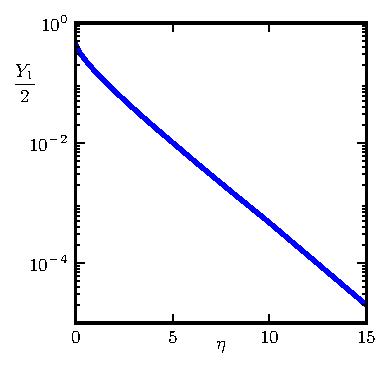
\includegraphics{Fig1}
		\caption{The function of the Knudsen layer \(Y_1(\eta)\) for a hard-sphere gas}
		\label{fig:Y1}
	\end{minipage}
	\quad
	\begin{minipage}{.48\textwidth}
		\centering
		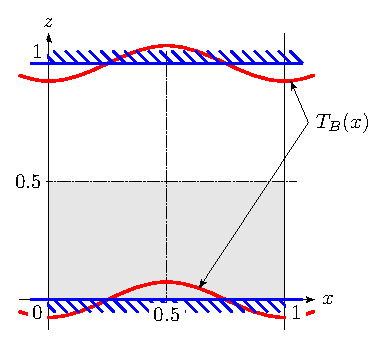
\includegraphics{Fig2}
		\vspace{13pt}
		\caption{Geometry of the problem with two parallel plates}
		\label{fig:geometry}
	\end{minipage}
\end{figure}

Generally, for \(\Kn\to0\), gas is not described by the heat-conduction equation~\eqref{eq:heat_equation}.
Equation~\eqref{eq:asymptotic3} converges to it only in the special case \(u_{i1} = 0\).
We can identify three reasons why this condition is not met:
\begin{enumerate}
	\item The boundary moves with the infinitesimal velocity: \(u_{wi} = u_{w1i} k\)~\cite{GhostEffect}.
	\item The boundary temperature is nonuniform (thermal creep flow)~\cite{Bobylev1996}.
	\item The isothermal surfaces are not parallel (nonlinear thermal-stress flow)~\cite{Kogan1976}:
		\begin{equation}\label{eq:equilibrium}
			e_{ijk}\pder[T_0]{x_j}\pder{x_k}\left(\pder[T_0]{x_l}\right)^2 = 0.
		\end{equation}
\end{enumerate}

The first two cases are directly determined by the boundary conditions,
and the third one has only an implicit impact from them.

\section{Numerical simulation}

\begin{figure}[ht]
	\centering
	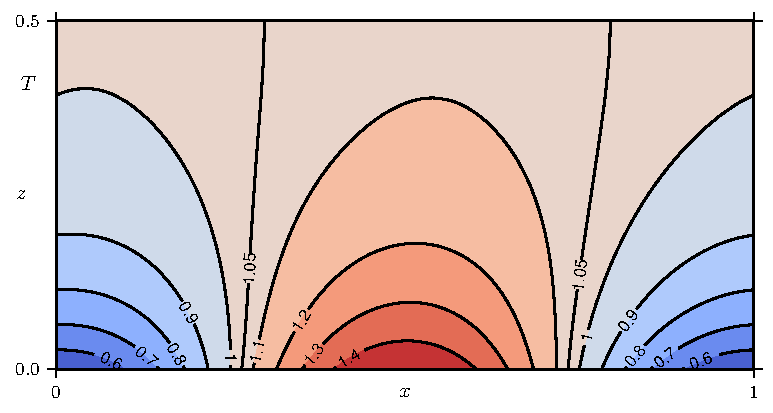
\includegraphics{Fig3}
	\caption{The temperature field \(T\), obtained from the asymptotic theory}
	\label{fig:moving:T_asym}
\end{figure}

\begin{figure}[ht]
	\centering
	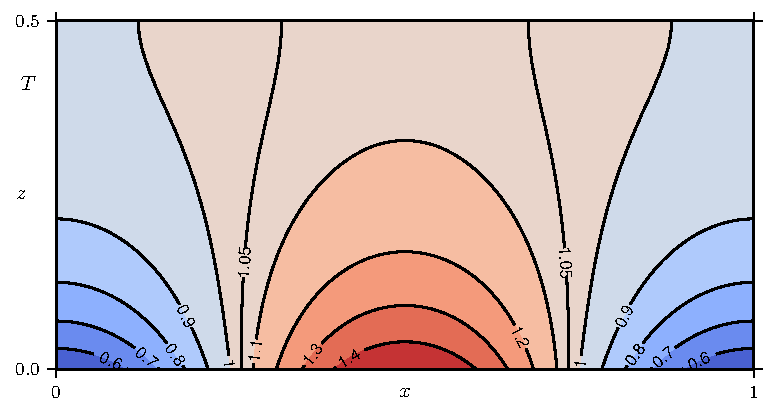
\includegraphics{Fig4}
	\caption{Temperature field \(T\), obtained from the heat-conduction equation}
	\label{fig:moving:T_heat}
\end{figure}

Special solver of the system~\eqref{eq:asymptotic1}--\eqref{eq:asymptotic3}
has been developed based on open source CFD toolbox OpenFOAM\textregistered{}~\cite{OpenFOAM1998},
which uses the finite-volume approach for evaluating partial derivatives.
The continuity equation~\eqref{eq:asymptotic1} together with the momentum equation~\eqref{eq:asymptotic2}
is solved with the commonly used implicit conservative algorithm SIMPLE~\cite{SIMPLE}.
A detailed description of this scheme for gas mixtures can be found in~\cite{Laneryd2007}.
Unstructured grids are generated with open source package GMSH~\cite{GMSH}.

All transport coefficients are taken in compliance with the hard-sphere model.
Complete diffuse reflection is assumed from solid surfaces.

Nonuniform spatial grids are condensed in areas with large gradients of macroscopic variables.
The residual of the solution for all considered problems does not exceed \(10^{-6}\).

\subsection{Gas between two parallel plates}

Consider a plane periodic geometry shown in Fig.~\ref{fig:geometry}.
The gas is placed between two infinite parallel plates
that have a sinusoidal distribution of the temperature
\begin{equation}
	T_w = 1-\alpha\cos(2\pi x).
\end{equation}
Lower plate moves relative to the top with the velocity
\begin{equation}
	u_{wi} = (\beta\Kn,0,0).
\end{equation}

We consider the special case:
\[ \alpha=1/2, \quad \beta = 1. \]

Due to the problem symmetry computational domain represents a rectangle \(0<x<1, 0<z<1/2\)
(a gray background in Fig.~\ref{fig:geometry}).

\begin{figure}
	\centering
	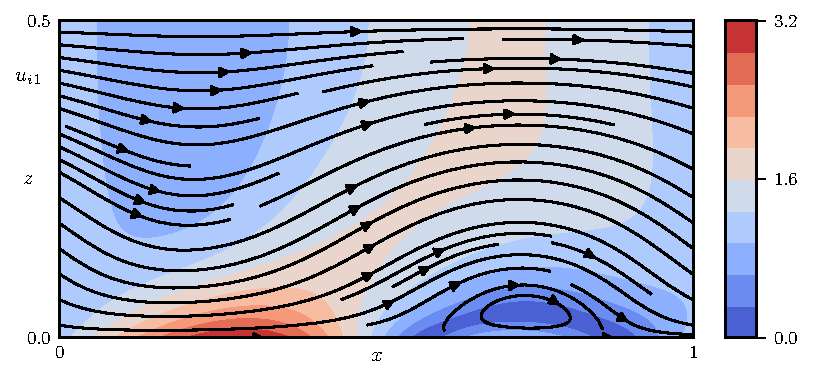
\includegraphics{Fig5}
	\caption{The fluid-dynamic part of the velocity field \(u_{i1}\)}\label{fig:moving:fluid}
\end{figure}

\begin{figure}
	\centering
	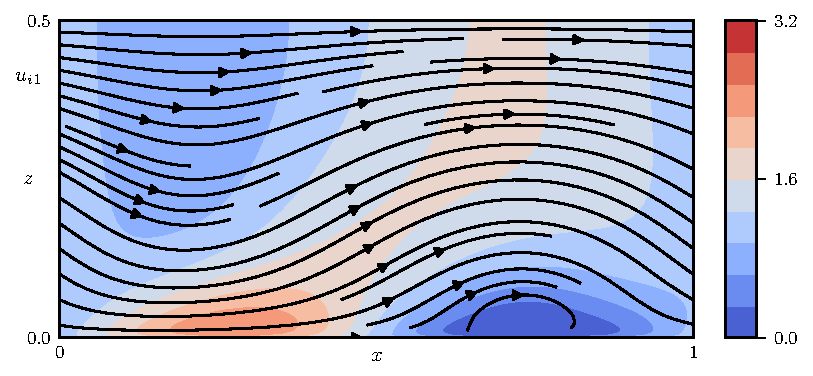
\includegraphics{Fig6}
	\caption{The velocity field \(u_{i1}\) with the Knudsen layer correction for \(\Kn=0.01\)}\label{fig:moving:kn001}
\end{figure}

The resulting temperature distribution in the continuum limit (Fig.~\ref{fig:moving:T_asym}) is shown
in comparison with the solution of the heat-conduction equation (Fig.~\ref{fig:moving:T_heat}).
When \(k\to0\) classical solution is seen to have a qualitative distinction from the kinetic one: 
the former comprises symmetry in the isothermal lines.

The velocity field \(u_{i1}\) is shown in Fig.~\ref{fig:moving:fluid} and Fig.~\ref{fig:moving:kn001}.
The Knudsen layer correction~\eqref{eq:bound:v_K} is taken into account in the latter figure.
We see that for small \(k\) the gas flow occurs in the thin Knudsen layer near the solid surface
directed along boundary temperature gradient.
This effect of the first order of \(k\) is called \textit{thermal creep flow}.

In the continuum limit the velocity field tends to zero:
\[ u_i = u_{i1}k + O(k^2) \to 0, \quad k\to0, \]
however \(u_{i1}\) remains finite and transforms the temperature field through~\eqref{eq:asymptotic3}.

Moreover, it is important to note that the solution is very sensitive to the mutual velocity of the plates.
Infinitesimal \(u_w\) has also the finite impact on the temperature field through \(u_{w1}\).

\subsection{Gas between two cylinders and spheres}

\begin{figure}
	\centering
	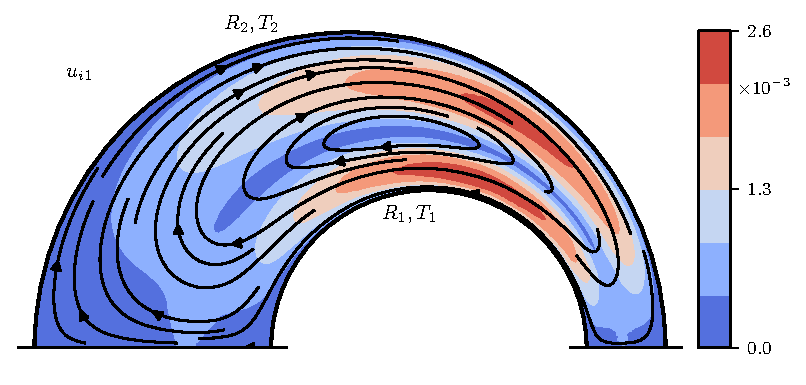
\includegraphics{Fig7}
	\caption{Stationary field \(u_{i1}\) between two noncoaxial cylinders}\label{fig:cylinders}
\end{figure}

\begin{figure}
	\centering
	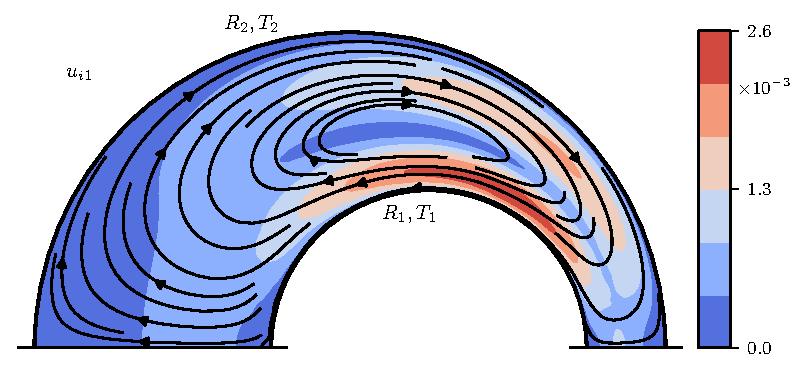
\includegraphics{Fig8}
	\caption{Stationary field \(u_{i1}\) between two nonconcentric spheres}\label{fig:spheres}
\end{figure}

Now consider the case of the temperature gradient absence in the surrounding bodies at rest.
As stated above, even under such boundary conditions convection flow can emerge
due to nonparallelism of the isothermal surfaces~\eqref{eq:equilibrium}.
This phenomenon has been called the \textit{nonlinear thermal-stress flow} and first described in~\cite{Kogan1971}.
The nonlinear origin of this effect in the first order of the Knudsen number is relevant,
because a linear thermal-stress flow appears only in the following order of smallness \(O(k^2)\).

This type of convection has a significant feature. It can occur in weightlessness
whereas a finite gravity field is necessary for the conventional convection excitation.

Consider two cylinders of radius \(R_1 = 1\) and \(R_2 = r\)
with temperatures \(T_1 = 1\) and \(T_2 = \alpha\), respectively.
The cylinder axes are parallel; the distance between them is equal to \(d\).

Fig.~\ref{fig:cylinders} presents the results of numerical simulation for the particular case:
\[ r = 2, \quad d = 1/2, \quad \alpha = 2. \]
The resulting velocity field \(u_{i1}\) is much weaker than in the previous problem,
so it has no noticeably visible influence on the temperature distribution.

Together with cylinders, nonconcentric spheres can be simulated in the same geometry.
In this case, the velocity pattern becomes as in Fig.~\ref{fig:spheres}.

\subsection{Gas between two elliptical cylinders}

\begin{figure}
	\centering
	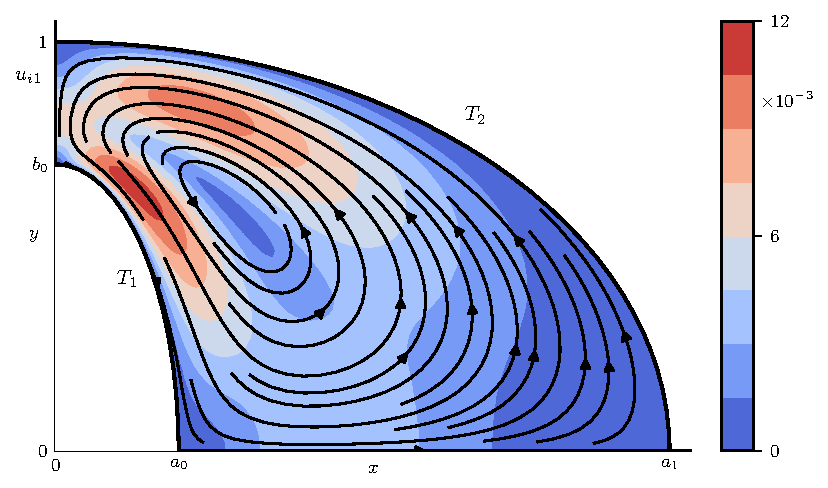
\includegraphics{Fig9}
	\caption{Stationary field \(u_{i1}\) between coaxial elliptical cylinders}
	\label{fig:elliptic}
\end{figure}

Consider the last problem in which the gas is placed between two coaxial elliptical cylinders
in such a way that the major axes of the ellipses in cross section are perpendicular.
Let the semi-minor axis of the outer cylinder be the characteristic length, while the semi-major one is \(a_1\).
The semi-axes of the inner ellipse are \(b_0\) and \(a_0\) in length, respectively.
The temperatures are equal to \(T_1 = 1\), \(T_2 = \alpha\) again.

We consider the special case:
\[ a_1 = 1.5, \quad a_0 = 0.3, \quad b_0 = 0.7, \quad \alpha = 2. \]

\begin{figure}[ht]
	\centering
	\begin{minipage}{.48\textwidth}
		\centering
		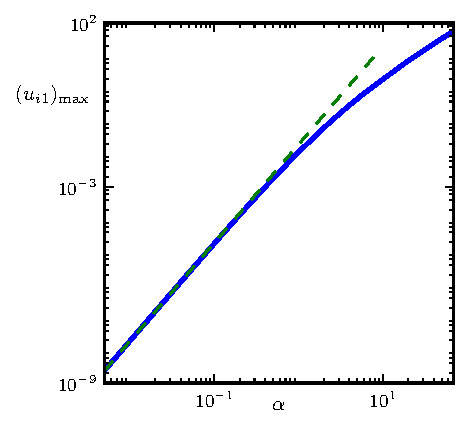
\includegraphics{Fig10}
		\caption{The maximum magnitude of \(u_{i1}\) versus the temperature ratio of the cylinders \(\alpha\)}
		\label{fig:maxU}
	\end{minipage}
	\quad
	\begin{minipage}{.48\textwidth}
		\centering
		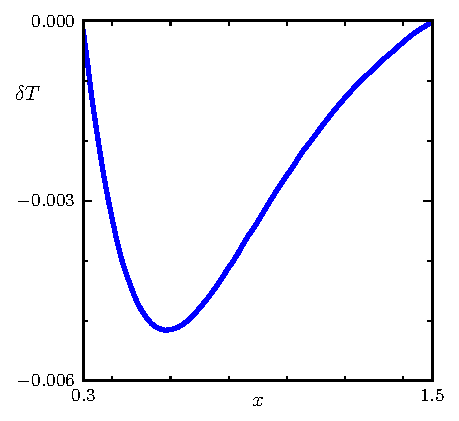
\includegraphics{Fig11}
		\caption{The difference in temperature fields \(\delta T\) along the \(x\) for \(\alpha = 5\)}
		\label{fig:deltaT}
	\end{minipage}
\end{figure}

Numerical simulation of a rarefied gas using the DSMC method in the current geometry
for a wide range of Knudsen numbers \(0.1\le\Kn\le5\) can be found in~\cite{SoneCoaxial}.

Calculation of such problems on the modern personal computer takes several minutes,
that allows you to quickly perform parametric studies as well. As an example,
the maximum magnitude of \(u_{i1}\) as a function of \(\alpha\) is shown in Fig.~\ref{fig:maxU}.
For small \(\alpha\) this relation satisfies the cubic law:
\begin{equation}
	\mathrm{max}(u_{i1}) \propto \alpha^3.
\end{equation}

Finally, Fig.~\ref{fig:deltaT} illustrates the appropriate discrepancy between the temperature fields
obtained from the asymptotic theory and the heat-conduction equation
\[ \delta T = T_\mathrm{asym} - T_\mathrm{heat} \]
along the major axis of the outer cylinder.

\section{Conclusion}

The Navier--Stokes set of equations is valid in the presence of a strong convection.
However, if the \(\mathrm{Re} \sim 1\) and the temperature variation in the gas is large
it ceases to be correct. So-called Burnett stress terms (higher-order terms of gas rarefaction)
begin to play a significant role in the gas behavior.
In this case, the asymptotic analysis of the Boltzmann equation arrives on the scene and yields
the correct set of equation solved in the present paper.

It is worth to mention about a surprising property of the derived system. It is the ghost effect
in the continuum limit. That is, in the limit when the Knudsen number vanishes,
the gas flow vanishes in proportion to the Knudsen number. However, this infinitesimal flow
has a finite effect on the temperature field.

Currently, there is a lot of CFD platforms provides comprehensive capabilities for
numerical simulation of the Navier--Stokes equations, but the present fluid-dynamic
set of equations remains in the shadow. Thus, the paper aims to
draw more attention for the CFD scope extension.

The key result of the present work consists in the developed universal solver for
the described set of equations and proper boundary conditions. It makes possible to
simulate all kind problems for arbitrary geometry in high speed and precision.
Calculations can be carried out both on a single personal computer and on a cluster.
The solver owes so much its important advantages to open-source platform OpenFOAM\textregistered{}
that served as the basis for the compact implementation of the utilized numerical methods.

The numerical examples examined above clearly demonstrate some temperature effects of
a slightly rarefied gas lying outside the scope of the Navier--Stokes set of equations:
the thermal creep flow and the nonlinear thermal-stress flow.

\bibliographystyle{spmpsci} % spbasic, spmpsci, spphys
\bibliography{springer}

\end{document}


